\chapter{Jolie Module System}

In this chapter, we present the module system for Jolie.
Similarly to how we presented python module system, we will walk-though the definitions, components, import mechanism, and lastly the redesign of Jolie's code file layout.

\section{Definitions}

Before diving into the details, it is beneficial to define a definition of components in a module system. In Jolie:

\begin{itemize}
    \item
          A \texttt{symbol} is a declaration of file level definition AST node. Symbol target is defined along with a module target in the import statement to specify which definition node it to be imported.
    \item
          A \texttt{module} is defined as a Jolie execution code in the file system. A module is a file contains symbols and the execution target for running the jolie code.
    \item
          A \texttt{package} is defined as either a directory in the file system or a file. A package role in the jolie module system is a place to hold the modules and can be part of the module target. A file with \texttt{.jap} extension, the Jolie's JAR-like achieve. is consider as a package which it's entry can be referred as a module.
\end{itemize}


\section{Import Statement}

An import statement enables the capability of importing a symbol from an external module. The declaration of an import statement consists of two specifiers, the module target and the target symbols, each used in different phases of import statement execution, the module lookup process, and the symbol binding process. Any error that occurs during the execution of an import statement, such as importing a restricted symbol or undefined symbol in the target module, will terminate the interpreter's execution.

The syntax for an import statement is shown in figure ~\ref{fig:jolie-import-stmt-syntax}.

\begin{figure}[ht]
    \begin{framed}
        \begin{grammar}
            <importStmt>
            ::= `from' <importingTargetModule> `import' <importingTargetSymbols>

            <importingTargetModule> ::= ( `.' )* ( <dottedName> | `.' )

            <dottedName>
            ::= <NAME> ( `.' <NAME> )*

            <importingTargetSymbols> ::=  `*' | <importAsNames>

            <importAsNames>
            ::= <importAsName> ( `,' <importAsName> )*

            <importAsName>
            ::= <NAME> ( `as' <NAME> )?

            <NAME> ::= <ID>
        \end{grammar}
    \end{framed}
    \caption{Jolie import statement syntax }
    \label{fig:jolie-import-stmt-syntax}
\end{figure}

The module target specifier used to guide the location where the importing module resides. Jolie import system uses a dot(.) as a path separation to the importing module. Each identifier before last defines the packages and sub-packages where the importing module resides, while the token at the end represents the importing module name. A leading dot designates Jolie import mechanism to perform a relative path lookup.

The second part of the import statement, target symbols, is a list of importing symbol names defined in the target module with an optional qualified name to bind to the local execution environment denoted by using 'as' keyword. For the current implementation of import statement wildcard import doesn't support importing with a qualified name (as).

\section{Symbol and Symbol Table}

The Symbol Table is a well-known data structure in programming languages. Generally, it is used as a truth table of reference between a named declaration, or symbol, associated with the source code. The term symbol refers to unique entities defined and used in the execution environment; the defined entities are such as variable names, function names, classes, and so on.
The Symbol Table is responsible for maintaining a data structure of this information and its description, such as the occurrences, declaration scope, and type. This data structure is useful throughout the program execution lifecycle, such as the analysis tasks and the optimization.

For the module system in Jolie, the Symbol Table is implemented with a hash table and associated with a single module.
The symbol contains essential information for performing binding in later stage this include: symbol name, scope, access modifier, and a pointer to abstract syntax node.
Scope indicates the location of the declaration node of the particular symbol, either internal or external; internal symbol specifies that the symbol definition declared within the module; on the contrary, external symbol, created from an import statement, determine that the interpretation defined from the external source.
An access modifier defines the accessibility of a symbol from the external module. It can be defined as \textbf{public}, which indicate that the symbol is accessible from external modules and allows to be imported. On the contrary, \textbf{private} prohibits access from the external module. A symbol is set to \textbf{public} by default; it can be defined as private by annotate a \textbf{private} keyword before the declaration of a symbol.

As the introduction of the symbol table, we have the definition of the abstract syntax node as defined in ~\ref{sec:jolie-def} and, additionally, the Service node, implemented as a newly added symbol. The Service node is a new abstract syntax node of Jolie for declaring a service, which we will get back to in later sections.

The construction of the symbol target consists of two stages. During the first stage, definition nodes are visited and pushed as a new entry in the symbol table. After this stage, every symbol defined within the module is bound to an abstraction node. In the second stage, a simple name lookup assigns the entry of an external module record, the corresponding abstract syntax node to the referring module's symbol table.

\begin{figure}[ht]
    \begin{subfigure}[b]{\textwidth}
        \lstset{language=Jolie,
            style=codeStyle,
            numbers=left,
            firstnumber=1
        }
        \begin{lstlisting}[frame=tlrb,
            basicstyle=\footnotesize]{symboltable.ol}
from C import *
from .B import b_type as b_imported
type A {
    a_type: int
}
private type from_b: b_imported
\end{lstlisting}
    \end{subfigure}
    \begin{subfigure}[b]{\textwidth}
        \begin{tabular}{ |c|l|l|l| }
            \hline
            Symbol name & scope        & privacy & binding abstract syntax \\
            \hline
            C*          & external(C)  & private & NONE                    \\
            b_imported  & external(.B) & private & NONE                    \\
            A           & local        & public  & $<$ type: A $>$         \\
            from_b      & local        & private & $<$ type: from_b $>$    \\
            \hline
        \end{tabular}
    \end{subfigure}
    \caption{Jolie code and its Symbol table}
    \label{fig:jolie-ex-symbol-table}
\end{figure}

From figure ~\ref{fig:jolie-ex-symbol-table} which demonstrates the construction of Symbol table.
There are three entries that get created at the first step of the symbol table creation. The detail of each symbol is the following:

\begin{itemize}
    \item \texttt{C*}, originated from an import statement, is instantiated as an \texttt{external(C*)}, which determines that the definition node is referring to an external source module named B. In this first step, the symbol name gets assigned as a unique name.
    \item \texttt{b_import}, originated from an import statement, is instantiated as an \texttt{external(.B)} which determines that the definition node is referring to an external module named B at a relative location with respect to the execution node.
    \item \texttt{A}, defined within the local execution is a local scope symbol with the \textbf{public} as the default privacy.
    \item \texttt{from_b}, has the keyword \textbf{private} before the declaration; thus, this symbol cannot be imported by others.
\end{itemize}

After this step, the partially created symbol table of the module is created. This partially filled symbol table has information on the syntax node defined within its module. The external-scope symbols are left without pointers to their binding abstract syntax node. To fully fill this field, we can simply perform a lookup on the symbol table of the module target that the declaration is originated from.

Consider figure ~\ref{fig:jolie-ex-symbol-table-completed} which defines a symbol of module \texttt{C} and the completed symbol table from previous example. Entry \texttt{C*} get replaced by the exposed symbol in its module.

\begin{figure}[ht]
    \begin{subfigure}[b]{\textwidth}
        \begin{tabular}{ |c|l|l|l|l| }
            \hline
            Source              & Symbol name & scope        & privacy & binding abstract syntax        \\
            \hline
            \multirow{3}{*}{C}  & C1          & local        & public  & $<$ type: C1 $>$               \\
                                & C2          & local        & private & $<$ type: C2 $>$               \\
                                & CIface      & local        & public  & $<$ interface: CIface $>$      \\
            \hline
            \multirow{4}{*}{.B} & C1          & external(C)  & private & $<$ type: C1 $>$ in C          \\
                                & CIface      & external(C)  & private & $<$ interface: CIface $>$ in C \\
                                & b_imported  & external(.B) & private & $<$ type: b_type $>$ in B      \\
                                & A           & local        & public  & $<$ type: A $>$                \\
                                & from_b      & local        & private & $<$ type: from_b $>$           \\
            \hline
        \end{tabular}
    \end{subfigure}
    \caption{Jolie Symbol table after completion}
    \label{fig:jolie-ex-symbol-table-completed}
\end{figure}

\subsubsection*{Module Record}

From here, we can define a new abstraction object in the Jolie interpreter ecosystem, considering that the symbol table is a representation of symbol usages in a module, and a module is parsed into a single abstract syntax tree node. The Module Record is an object consisted of an AST and symbol table of a module it's referred to.


\section{ Name Resolution }

The introduction of Symbol Table allows Jolie interpreter parses the definition referencing in abstract syntax by using lazy evaluation strategy. This benefits Jolie developer by allowing symbol referencing without worry about definition order. To illustrate the problem Jolie had before, consider the following source code:
\begin{listing}[ht]
    \lstset{language=Jolie,
        style=codeStyle
    }
    \begin{lstlisting}[frame=tlrb]{definitionOrder.ol}
define bar{
    foo
}

define foo {
    bar
}
\end{lstlisting}
\end{listing}

The execution is failed to parse since the parser cannot find a procedure definition \texttt{foo} when attempt to parse token foo inside procedure \texttt{bar}.
By introducing name resolution to the current workflow, it is possible to write and use definition without a concern on the order. During parsing phase, Jolie interpreter assigns an empty named symbol object which will be resolved to an expected abstract syntax by performing name resolution.

\section{ Module Crawling }

Module Crawling is a process of locating and parsing the dependencies of the execution module.
The module crawler is essential for the Jolie module system in such a way that it constructs a set of required module records for the execution of a program.

The crawling process takes an initial module record and scans for the dependent modules. After a dependent module has been found, it is parsed and scanned for its dependent modules. These dependencies are stored in a queue data structure with a cache. The module crawler repeatedly performs this procedure until every dependent module has successfully parsed into the Symbol Table. The algorithm for this function is defined in procedure \texttt{crawl} in algorithm ~\ref{algo:crawl}.

\begin{algorithm}
    \begin{algorithmic}[1]

        \Require{A crawling module record $root$}
        \Ensure {Module records required for the execution $result$}

        \Procedure {Crawl}{$root$}

        \State $Q\gets \Call{FetchDependency}{root}$ \Comment{module to crawl}
        \State \Call{$result.put$}{$root$} \Comment{add root to result}

        \While{$Q$ is not empty}
        \State $module\gets \Call{Q.poll}{}$

        \If{$module$ in $result$}
        \textbf{continue} \Comment{record is already parsed}
        \EndIf

        \State $record\gets$ \Call{parse}{$module$} \Comment{parse source into a module record}

        \State $deps\gets \Call{FetchDependency}{record}$
        \ForAll {$d$ in $deps$}
        \If{$d$ not in $Q$}
        \State \Call{$Q.add$}{$d$}
        \EndIf
        \EndFor
        \State \Call{$result.put$}{$record$} \Comment{add record to result}

        \EndWhile
        \EndProcedure

        \Function {FetchDependency}{$mr$}
        \State $deps\gets$ new list
        \ForAll{$s$ in $mr$'s external scope symbols}
        \State $moduleTarget\gets$ module target of $s$
        \State $source\gets \Call{find}{moduleTarget}$ \Comment{find operation by finder}

        \State \Call{$deps.insert$}{$source$}
        \EndFor

        \State \textbf{return} $deps$ \Comment{list of dependency module for $mr$}
        \EndFunction

    \end{algorithmic}
    \caption{Jolie module system's module crawling algorithm}
    \label{algo:crawl}
\end{algorithm}
\FloatBarrier

The Module finding is performed by a component of the module crawler called finder. The current implementation of Jolie module system has two types of finders, which define different strategies to locate a module. The Absolute Finder performs a lookup at a set of defined path locations. The Relative Finder performs a search from a relative path to the import statement caller. The finder is responsible for finding an imported module and making sure that the import target exists in the file system. If the finder failed to retrieve the module's information, the interpreter raises a ModuleNotFound error and stops its execution.

\subsection{ Absolute Path Resolution }

The absolute import, which performs a search for the module at a defined path location, is used for importing a library that does not reside in the package-specific modules. The use case for such an import resolution strategy is that of built-in modules.

The Absolute Path Finder performs a lookup in two different locations. The working directory of the execution process is the first place to perform a lookup, where the finder directly tries to resolve the target module. Then, it continues to the directory \texttt{lib} to look for \texttt{first.jap} where \texttt{first} is a first token defined in module target. Lastly, the finder will perform module lookup to the extensible list of directories defined in a special path called \texttt{packLib}. It contains a path to built-in libraries and can be extended through command-line arguments. The procedure for the absolute path resolution is shown in algorithm ~\ref{algo:absolutePath}:

\begin{algorithm}[H]
    \begin{algorithmic}[1]
        \Require{A module target $target$}
        \Require{A working directory of execution process $wdir$}
        \Require{A list of package directories $libs$}

        \Ensure {A location to the existed module in file system}

        \Procedure {find}{}
        \State $P\gets$ \Call{$target.split$}{`.'} \Comment{package/module tokens}
        \State $first\gets P[0]$ \Comment{first element of $P$}
        \State $rest\gets P[1...]$ \Comment{elements after first of $P$}

        \State $module \gets$\Call{resolve}{$wdir$, $P$}
        \If{$module$ existed}
        \State \textbf{return} $module$ \Comment{target module located in $wdir$}
        \EndIf

        \State $japPack \gets$\Call{resolve}{$wdir$, `lib', $first$}
        \If{$japPack$ existed and has jap extension}
        \If{$japPack$ has $rest$ as a entry}
        \State \textbf{return} $japPack$
        \EndIf
        \EndIf

        \ForAll{$lib$ in $libs$}
        \State $module \gets$\Call{resolve}{$lib$, $P$}
        \If{$module$ existed}
        \State \textbf{return} $module$ \Comment{target module located in $lib$}
        \EndIf
        \EndFor

        \State \textbf{return} None \Comment{lookup failed}

        \EndProcedure

    \end{algorithmic}
    \caption{Jolie module system's module finding algorithm for an absolute import}
    \label{algo:absolutePath}
\end{algorithm}

\begin{figure}[ht]
    \begin{forest}
        for tree={
        font=\ttfamily,
        grow'=0,
        child anchor=west,
        parent anchor=south,
        anchor=west,
        calign=first,
        edge path={
                \noexpand\path [draw, \forestoption{edge}]
                (!u.south west) +(7.5pt,0) |- node[fill,inner sep=1.25pt] {} (.child anchor)\forestoption{edge label};
            },
        before typesetting nodes={
                if n=1
                    {insert before={[,phantom]}}
                    {}
            },
        fit=band,
        before computing xy={l=15pt},
        }
        [.
            [lib
                    [someLib.jap
                            [module.ol]
                    ]
            ]
            [packages
                    [somePackage.ol]
            ]
        main.ol
        ]
    \end{forest}

    \lstset{language=Jolie,
        style=codeStyle,
        numbers=left,
        firstnumber=1
    }
    \begin{lstlisting}[frame=tlrb]{import-statement-absolute.ol}
from someLib.module import componentA
from packages.somePackage import componentB
from console import consoleService
\end{lstlisting}
    \caption{Demonstration of absolute import usage in Jolie's module system}
    \label{fig:jolie-absolute-import}
\end{figure}
Consider figure ~\ref{fig:jolie-absolute-import}, which shows a working-directory tree representation and a working-code snippet in \texttt{main.ol}, demonstrates the relation between module targets and the actual working directory structure. The import statement defined at the first line demonstrates an example of importing a jap archive file, while the second line is resolved into a ./packages/somePackage.ol. Lastly, the last line is an example of importing a built-in module \texttt{console}.


\FloatBarrier


\section{Jolie Module System Implementation}

In this section, we are looking into the Jolie interpreter's workflow for support of the module system. After discussions on necessary components for an import mechanism in Jolie, we are ready to revisit the flow we had mentioned before in section ~\ref{sec:jolie-implementation}; bold typesetting is used for indicating the additional flow.

\begin{enumerate}
    \item The command-line arguments for the interpreter configuration are parsed. And the target execution file is located.
    \item The source code gets parsed by the parser, where the \textbf{module record of execution target is created}.
    \item \textbf{The dependent modules gets crawled by Module Crawler, given the initial module record.}
    \item \textbf{Revisit symbols in symbol tables to link the reference between an external SymbolNode and the target reference node defined in the importing module.}
    \item \textbf{Perform symbol name resolution to link the Symbol to the appropriate definition node}
    \item The program's component nodes in AST get semantically verified.
    \item Transform abstract syntax tree \textbf{of the main procedure in main service} to the interpretation tree or the executable runtime object.
    \item Initialize the Communication Core from incoming communication ports description, the service is ready to receive an incoming message after this process is finished.
    \item Initialize the embedding services, and the communication configuration processes for outgoing communication port are executed.
    \item The runtime executes the main procedure definition process.
\end{enumerate}.

The resolving alias type process, which was performed during the semantic verification phase, is no longer needed since the symbol name resolution process already handles the task.
Another notable change in the workflow is the target of OOIT creation, where we used to pass the whole AST of a Jolie file.
This is no longer be the case since our definition of a Jolie executable file has changed from being a representation of a service into a module.
Hence, we introduce a \textit{service definition} as an input of the interpretation tree creation process.

\section{Service Node}

As the adjustment of Jolie execution file definition has changed, the file structure layout has to be modified as well.  At top level definitions, the abstract syntax of definition nodes such as types and interfaces are remained. But the service related syntax nodes such as behavioral and instruction on deployment has to be moved into a proper scope which represent a definition of a service. This lead to an introduction of a new syntax node in Jolie module system; such node is called a \textit{Service Node}.

In the implementation level, Service Node is responsible for storing deployment instructions and behaviors of a service. It may optionally accepted a parameter, which can be passed to during embedding process.
With this change, we can use the import mechanism to import and embed a service easily, by specify a service as an identifier, rather than using string defining a path as before.
The definition of service node also covers declaration of the external technology service, in particular, the one that we used in existed embedding mechanism ~\ref{sec:embedded}.
In this new implementation of foreign technology service node, it can be view as a special type of jolie service which can interact with foreign technology.
The grammar for Jolie module system is defined in figure ~\ref{fig:jolie-servicenode-grammar}

\begin{figure}[h]
    \begin{framed}
        \begin{grammar}
            <jolie> ::= <importStmt>* <definitions>*

            <definitions> ::= `private'? <definition>

            <definition> ::=  <typeDefinition>
            \dots
            \alt <serviceNode>

            <serviceNode> ::= `service' <technology>? <ID> <param>? \\ `{' <deplInstruction>* `main' `{' <behaviors> `}'`}'

            <technology> ::= <java> | <javascript> | <jolie>

            <jolie> ::= `Jolie'

            <java> ::= `Java' `(' <StringLiteral> `)'

            <javascript> ::= `Javascript' `(' <StringLiteral> `)'

            <param> ::= `(' <ID> : <paramType> `)'

            <paramType> ::= <ID>
        \end{grammar}
    \end{framed}
    \caption{Jolie Service Node Grammar}
    \label{fig:jolie-servicenode-grammar}
\end{figure}

\begin{listing}[h]

    \lstset{language=Jolie,
        style=codeStyle,
        numbers=left,
        firstnumber=1
    }
    \begin{lstlisting}[frame=tlrb, caption= {Jolie Service Node Example}, label={list:jolie-servicenode} ]{servicenode-jolie}
interface prefixerIface{
    requestResponse: prefix(string)(string)
}

service prefixService ( prefix: string )  {
    
    inputPort IP {
        interfaces : prefixerIface
        protocol: sodep
        location : "socket://localhost:3000"
    }

    execution{ concurrent }

    main {
        [prefix(req)(res){
            res = prefix + req
        }]
    }
}
    \end{lstlisting}
\end{listing}

Listing ~\ref{list:jolie-servicenode} illustrates a code snippet for declaration of service node, \textit{prefixService}. The service accept a string as a parameter 

 It is in clear view that the definitions that direct the behavior of a service is encapsulate in a Service Node called \textit{mulService}, This service accepted a value of integer, which determine a second factor of multiplication operation. It is also exposes the communication channel through an interface \textit{mulIface}, which is declared at file level scope and can be imported by an external module.

\FloatBarrier

\subsubsection*{Jolie Script}

Running a Jolie interpreter instance involve a translation of a service abstraction into an OOIT as one of the execution process.
As we have changed the definition of a service, in particular, a Jolie executable file is no longer represent a service, rather becoming a module.   
We also introduce an encapsulation of the service abstraction into a service node, which multiple can be defined within a single module.
For these reasons, making it ambiguous for an interpreter to decided which service node to be used as an translation target, it is essential to have a convention of target service node when a module is given as a execution target.
Hereby, we introduce the definition of an executable Jolie module so called \textit{Jolie script}.

<<<<<<< HEAD
A Jolie script is a module that included a service node named \texttt{main}. A main service node in Jolie script is a special declaration which is treated as a execution service by the interpreter. Moreover, it can also be used as an import target for the import statement.
=======
Jolie script, a main candidate for running Jolie program, is a module that included a service node named \texttt{main}. Considering the listing ~\ref{list:jolie-procedure-script} which is a rewritten version of the example we had before in ~\ref{list:procedure}, the only difference here is the behavior of the service is enclosed in a special service node named main. Which is a execution target when the script get pass to the command-line.
>>>>>>> a84fbad8850b6673ac4c54e3b347f48a75834b3b

\begin{listing}[h]
    \lstset{lan guage=Jolie,
        style=codeStyle
    }
\begin{lstlisting}[frame=tlrb, caption= {A Jolie script version of ~\ref{list:procedure}}, label={list:jolie-procedure-script}]{procedure-script-Jolie}
define doubleX{
    X = X * 2
}

service main {
    X = 5
    doubleX
    // now X == 10
}
\end{lstlisting}
\end{listing}

<<<<<<< HEAD
Consider figure ~\ref{list:jolie-procedure-script} which defined an equivalence outcome from ~\ref{list:procedure} but using a module system style. When running this script, the target interpretation of service uses main as a target execution even if there is multiple service node declared within a same file.
=======
It is worth mentioning that running a non Jolie script modules is prohibited and program will terminate during semantic verifying step.
>>>>>>> a84fbad8850b6673ac4c54e3b347f48a75834b3b

\subsection{Embedding Service Node}

An embedding mechanism is also extended into a service node. It enables implementation of service orchestration in 
A service node can be embedded 

\subsubsection{Parameterize Service}

\subsection{Backward compatibility}

Since Jolie module system is relatively new and cause a breaking change on the previous version, we decided to keep the backward compatible with the old syntax. If the interpreter detected old syntax or jolie file, the AST will be transform by moving all behavior and deployment instruction nodes into the newly created main Service Node while definition nodes will remain in top level definitions. The method of detecting old syntax is relatively easy, one of trivial method is to detect whether the AST contain an Procedure Definition named \texttt{main}.

\begin{algorithm}[h]
    \caption{TransformJolieCodeToModule}
    \label{algo:transfrom}
    \begin{algorithmic}[1]
        \Require{An abstract syntax tree of Jolie program $program$}
        \Ensure {An abstract syntax tree of Jolie Module $result$}

        \Procedure {transform}{}
        \State $moduleProgram\gets$ new list\Comment{new module's program node}
        \State $serviceProgram\gets$ new list\Comment{new new Service program node}

        \ForAll{$node$ in $program$}
        \If{$node$ is $Symbol$}
        \If{$node$ is $Procedure$ and $node$ named \texttt{`main"} or \texttt{`init"} }
        \State \Call{$serviceProgram.add$}{$node$}
        \Else
        \State \Call{$moduleProgram.add$}{$node$}
        \EndIf
        \Else{
            \If{$node$ is $ImportStatement$}
            \State \Call{$moduleProgram.add$}{$node$}
            \Else
            \State \Call{$serviceProgram.add$}{$node$}
            \EndIf
        }
        \EndIf
        \EndFor
        \State $serviceNode \gets$ new service node from $serviceProgram$
        \State \Call{$moduleProgram.add$}{$serviceNode$}
        \State $result \gets$ $moduleProgram$
        \EndProcedure

    \end{algorithmic}
\end{algorithm}
\subsection{Code example}

In this section, we introduce the reader to a simple example program of Jolie. The program emphasizes the capability of the module system by interchanging a service through common interface operation.  

The following code snippet is a hello-world example of the Jolie module system.

\begin{listing}[H]
    \lstset{language=Jolie,
        style=codeStyle,
        numbers=left,
        firstnumber=1
    }
    \begin{lstlisting}[frame=tlrb]{service-hello.ol}
from console import ConsoleService, ConsoleInterface

service main(){

    outputPort Console {
        interfaces: ConsoleInterface
    }

    embed ConsoleService() in Console

    main{
        print@Console("Hello")()
    }
}
\end{lstlisting}

\end{listing}

At line 1, we have an import statement to import the ConsoleService along with the interface exposed by its service. The ConsoleService is a build-in service that allows a Jolie program to communicate to the execution process system console. Afterwards, we declare a service node called main, with an outgoing communication Console that uses an operation in ConsoleInterface. At line 9, The communication port Console is later bound with the service ConsoleService through the embed statement. It resulted in an usable Console port which communicates internally with ConsoleService, without specification on the location or protocol parameter in its declaration.
In the main procedure, we invoke the operation \textit{print} through the output port Console. Executing this program results in \say{Hello} being printed at the process console.

\subsubsection{Service Injection Pattern}

Our last example describes a way to compose a simple service in the Jolie module system. Here, we can extend the previous example to an advanced scenario. Given a situation where we want to have our own workflow on the operation \textit{print}. We create a new service, \textit{PrinterService}, which exposes the operation \textit{print}, with a simple workflow of prefixing an incoming message before forwarding it to the system console.

\begin{listing}[H]
    \lstset{language=Jolie,
        style=codeStyle,
        numbers=left,
        firstnumber=1
    }
    \begin{lstlisting}[frame=tlrb]{printer.ol}
from console import ConsoleService, ConsoleInterface

interface PrinterInterface {
RequestResponse:
    print( undefined )( void )
}

service PrinterService() {

    execution { concurrent }
    
    inputPort IP {
        location: "local"
        interfaces: PrinterInterface
    }

    embed ConsoleService in new _Console

    main{
        [print(req)(res){
            res = "Printer receive: " + req
            print@_Console(res)()
        }]
	// omitted code
    }
}
\end{lstlisting}
\end{listing}

\begin{listing}[H]
    \lstset{language=Jolie,
        style=codeStyle,
        numbers=left,
        firstnumber=1
    }
    \begin{lstlisting}[frame=tlrb]{service-injection-hello.ol}
from console import ConsoleInterface
from .printer import PrinterService

service main(){

    outputPort Console {
        interfaces: ConsoleInterface
    }

    embed PrinterService() in Console

    main{
        print@Console("Hello")()
    }
}
\end{lstlisting}
\end{listing}

After the service has been defined, we only have to import and embed the \textit{PrinterService} instead of \textit{ConsoleService} of our last example. The client of this service will now use the operation \textit{print} of the \textit{PrinterService} and program results in \say{Printer receive: Hello} being printed.

Since the operation \textit{print} is commonly exposed by both services, thus, these two services are interchangeable for the operation \textit{print}. 

The module system extends the flexibility of Jolie services and allows the service developer to create a new system in a modular approach. In the next section, we will look at the practical Jolie module system implementation of the Circuit Breaker, which is one of the prominent microservices patterns \cite{nygard2007release}.

\FloatBarrier

\subsubsection{Microservice Pattern: Circuit Breaker}

In this section, we discuss an implementation of the circuit breaker pattern in Jolie and emphasize Jolie’s capability as a language for microservices. After the discussion on implementation source code, we also explore the integration of this application with the container technology, particularly Docker container.

The circuit breaker is a well-known pattern in the microservice architecture \cite{martin-2015-circuit, microservices.io-circuit}. It enables an application to proceed on a request properly on the situation of an arbitrary dependent service that has failed to progress. A possible application scenario of circuit breaker is where a network of services communicate with each other to build up a client’s response, and one of the services is taking a longer-than-usual processing time. This processing time can be a result of network latency. Otherwise, there might be a failure during the processing of a task, which cannot be foreseen by other services. The pattern increases the fault-tolerant of the whole system by monitoring the service behavior and prevents an unexpected failure from cascading to other services by performing a cutout action, just like the circuit breaker in the physical world.

A circuit breaker implementation in the microservices ecosystem is a proxy service between clients to a service. The circuit breaker monitors the request and counts the number of failures that happens through calls made to the destination service. If the number of failures reaches the threshold, it discards and returns a meaningful response for the client without attempting to make a call to the destination service. Later after a certain amount of time, on the invocation to the service, the circuit breaker slowly forwards the request again.

There are three states in circuit breaker which determine the state of calls made to the destination service. Firstly, the \textit{Closed} is a healthy state of the circuit breaker. At this state, every request for an operation will be passed to the service. Each failure occurred from the call, either internally from the service or the request timeout, the circuit breaker increases the counter.When the number of failures reaches the threshold number, the circuit breaker trips by changing its state to \textit{Open} and start a reset timeout. At this state, any request made to the destination operation is skipped by the circuit breaker as it is presumed that the destination service is down. The developer of the circuit breaker can design the fallback procedure, for example, return a cached response to the client or straightforwardly return an error response. After the reset timeout ticks, the circuit breaker changes its state to \textit{Half-Open}, where any call will be passed to the destination service. If the service responds without any error, the circuit breaker sets its state to \textit{Closed} or in a healthy state. Otherwise, the circuit breaker falls back to status \textit{Open} again. The states for a circuit status illustrate in the figure\ref{figure:circuit-breaker-state-diagram}. 

\begin{figure}
    \centering
    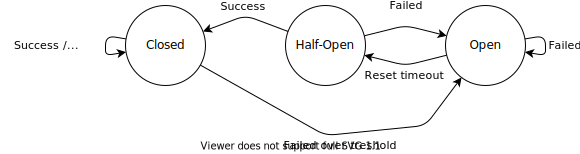
\includegraphics[width=\textwidth]{Doc-images-circuit-breaker.pdf}
    \caption{State diagram for circuit breaker service}
    \label{figure:circuit-breaker-state-diagram}
\end{figure}

Montesi and Weber have studied the implementation of circuit breaker pattern for Jolie application\cite{10.1145/3167132.3167427}, which extends a decorator pattern and sketches an implementation of circuit breaker pattern in Jolie. In our version, we exploit the capability of importing service to extend a single service with a circuit breaker extension service. We begin with a circuit breaker service, which is implemented as an extension service to be imported and embedded by others. We firstly define types and interfaces definitions for the circuit breaker, which is shown in figure.

Start with a circuit breaker service, which is implemented as an extension service to be imported and embedded by others. We firstly define types and interfaces definitions for the circuit breaker, as shown in figure ~\ref{list:circuit-breaker-def}. We required three interfaces for handling the operation as followed:
\begin{itemize}
    \item the \texttt{HTTPInterface} defines an operation for handling an communication between the circuit breaker to the client.
    \item The \texttt{CircuitBreakerServiceCallbackInterface}, defines an operation for handling an communication between the circuit breaker to the destination service.
    \item Lastly, \texttt{CircuitBreakerInternalInterface} defines the internal operation such as timeout for resetting the Opened state and request timeout handler. 
\end{itemize}

The client requests are handled through an HTTP protocol with a special configuration \textit{default}, which will be invoked as a default operation when the undefined operation is passed to the service.  field by assigning the service parameter. Figure ~\ref{list:circuit-breaker-component-diagram} demonstrated the interfaces exposed by the circuit breaker service.

\begin{figure}
    \centering
    \includegraphics[width=\textwidth]{Doc-images-circuit-breaker-service.pdf}
    \caption{Component diagram for the circuit breaker service}
    \label{list:circuit-breaker-component-diagram}
\end{figure}

Furthermore, we also define a type for configuring the service. As a proxy service, we require additional input from the embedder service, the exposing input location, and the target location. 
It is worth mentioning that we give the responsibility to importer service to configure \textit{location} of the communication channel. The source code for what we have mentioned so far is shown at figure ~\ref{list:circuit-breaker-def}

\renewcommand{\topfraction}{.85}
\renewcommand{\bottomfraction}{.7}
\renewcommand{\textfraction}{.15}
\renewcommand{\floatpagefraction}{.66}
\renewcommand{\dbltopfraction}{.66}
\renewcommand{\dblfloatpagefraction}{.66}
\setcounter{topnumber}{9}
\setcounter{bottomnumber}{9}
\setcounter{totalnumber}{20}
\setcounter{dbltopnumber}{9}

\begin{listing}[]
    \lstset{language=Jolie,
        style=codeStyle,
        basicstyle=\ttfamily\footnotesize
    }
    \begin{lstlisting}[frame=tlrb]{circuitbreaker-definitions.ol}
interface HTTPInterface{
    requestResponse:
        default(undefined)(undefined)
}

interface CircuitBreakerServiceCallbackInterface{
    requestResponse: callback(undefined)(undefined) throws UnexpectedError(string)
}

private interface CircuitBreakerInternalInterface{
    oneWay: reset(undefined)
}

type CircuitBreakerServiceParam : void {
    inputLocation: string
    outputLocation: string
}

service CircuitBreakerService (p : CircuitBreakerServiceParam) { 
    inputPort HTTPInput {
        protocol: "http" {
            default = "default"
        }
        location: p.inputLocation
        interfaces: HTTPInterface
    }
    outputPort DestService {
        location: p.outputLocation
        protocol: "sodep"
        interfaces: CircuitBreakerServiceCallbackInterface
    }
    inputPort SelfInput{
        location: "local"
        interfaces: CircuitBreakerInternalInterface
    }
    ...
}
\end{lstlisting}
\caption{Definitions and communication ports for the circuit breaker service}
\label{list:circuit-breaker-def}
\end{listing}

Next as shown in figure ~\ref{list:circuit-breaker-workflow}, we define procedures and workflow for each operation exposed by the circuit breaker. The procedures included in this service encapsulate the actions made for state transformation. We use a global state, a shared state lived in every session initiated by the service, to store the counter of error number and the flag of the current status of the circuit breaker.

\begin{listing}[]
    \centering
    \lstset{language=Jolie,
        style=codeStyle,
        basicstyle=\ttfamily\footnotesize
    }
\begin{lstlisting}[frame=tlrb]{circuitbreaker-port.ol}
// constants declaration
service CircuitBreakerService (p : CircuitBreakerServiceParam) {
    ...
    define closeCircuit {
        global.errorCount = 0
        global.status = STATUS_CLOSED
    }
    define resetCircuit {
        global.status = STATUS_HALFOPEN
    }
    define trip {
        global.status = STATUS_OPEN
        scheduleTimeout@Time( TIMEOUT_REQUEST{.operation="reset"} )( )
    }
    define handleError {
        if (global.status == STATUS_HALFOPEN){
            trip
        } else if (global.errorCount > ERROR_THRESHOLD){
            trip
        }
    }
    init {
        closeCircuit
    }
    main {        
        [ reset() ]{
            resetCircuit
        }
        [ default( request )( response ) {
            if ( global.status == STATUS_OPEN ){
                response = "CircuitOpen"
            } else {
                install( UnexpectedError =>
                    global.errorCount++
                    handleError
                    response = "ServiceError"
                )
                callback@DestService(request)(serviceRes)

                if (global.status == STATUS_HALFOPEN){
                    closeCircuit
                }

                response << serviceRes
            }
        }]
    }
}
\end{lstlisting}
\caption{Workflow for circuit breaker service}
\label{list:circuit-breaker-workflow}
\end{listing}

The \textit{trip} procedure defines the instruction set to turn on the circuit, which is determined by procedure \textit{handleError}. After modifying the state, it proceeds with scheduling the timeout request for state recovery, defined in \textit{resetCircuit}, by invoking the operation from build-in service \textit{time}
\footnote{Time service specification \url{https://jolielang.gitbook.io/docs/language-tools-and-standard-library/standard-library-api/time}}.

The circuit breaker's initialization begins with a call to procedure \textit{closeCircuit}, which sets the state of the circuit to \textit{Closed} state. Later in the main execution, the service exposes and waits for two operations \textit{reset} and \textit{default}. The \textit{reset} operation is responsible for turn an Opened state of the circuit breaker to \textit{Half-Opened} by calling \textit{resetCircuit} procedure defined above. The operation for handling client requests, \textit{default}, as mention above, is invoked whenever the client is passing a message to the circuit breaker and forward the request to the destination service. The workflow of operation can be described as the following:
if the state of the circuit breaker, return a response without passing the request to destination service.
Otherwise, forward the request to destination service, if there is an error occurrence, call the error handling procedure and return a response to the client.

After we have defined the CircuitBreaker proxy service, which can be imported and embedded by any service, we look into an example service \textit{AddService}, which integrates the CircuitBreaker extension to handle the possible error that might occur internally.

\begin{listing}[]
    \lstset{language=Jolie,
        style=codeStyle,
        basicstyle=\ttfamily\footnotesize
        }
    \begin{lstlisting}[frame=tlrb]{circuitbreaker-client.ol}
from .circuitbreaker import CircuitBreakerService, CircuitBreakerServiceCallbackInterface

type input: void{
    x : int
    y : int
}

interface calculatorIface {
    requestResponse: 
        add(input)(int)
}

service main {
    
    // definition of self ports to redirect the request

    inputPort fromCircuitBreaker{
        location: "socket://localhost:3001"
        protocol: "http"
        interfaces: CircuitBreakerServiceCallbackInterface
    }

    embed CircuitBreakerService( { 
        inputLocation = "socket://localhost:3000"
        outputLocation = "socket://localhost:3001" 
    } )

    execution { concurrent }

    main{
        [add(req)(res){
		...
        }]
        [callback(req)(res){
            if (req.operation == "add"){
                add@SelfOp({x = int(req.data.x) y = int(req.data.y)})(response)               
            }       

		    if (error){
	    		throw ( UnexpectedError )
		    } else {
                res << response
         	}                  
        }]
    }
}
\end{lstlisting}
\caption{Jolie implementation of a service embedding the circuit breaker service}
\label{circuitbreaker-client.ol}
\end{listing}

Our implementation of the circuit breaker embedder, as shown in figure ~\ref{circuitbreaker-client.ol}, requires defining an operation \textit{callback}, which receives a message from the circuit breaker and redirect the request to proper operation. In this case, the workflow includes checking the request operation from \textit{operation} field then forward the message to an internal input port, defined using \textit{local} scheme for location. After the call is complete, return the corresponding result to the circuit breaker.

We had demonstrated an implementation of the microservice architecture, the circuit breaker, using the new feature of the module system. The Jolie module system enables Jolie developer to create and compose multiple sole responsibility services and create a more complex application using the import mechanism.


